\section{Invarianter för studenters laborationsantal}

\subsection{Max en LHG per laboration ($\leq 1$)}
\subsubsection{Förslag på implementering}
\subsubsection{Bevis av korrekthet}

\subsubsection{Användarperspektiv}

\begin{figure}\label{fig:slack_series}
  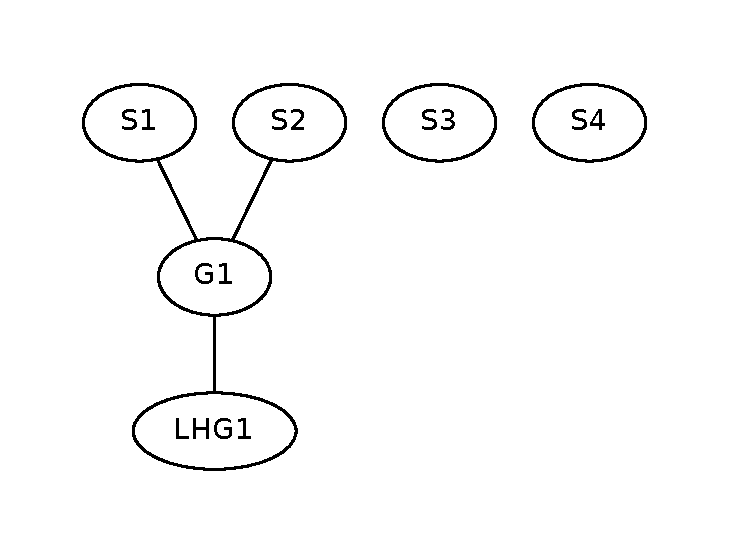
\includegraphics[width=7.0cm]{fig/labgroup/slack_add_1.pdf}        
  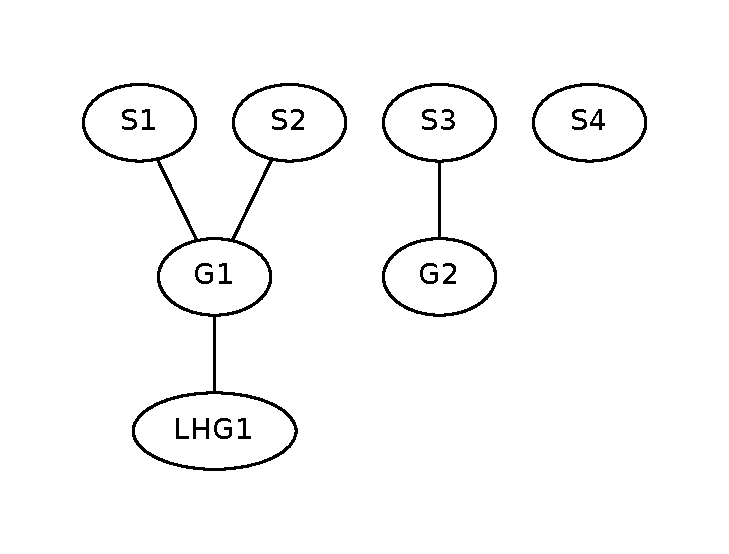
\includegraphics[width=7.0cm]{fig/labgroup/slack_add_2.pdf}        
  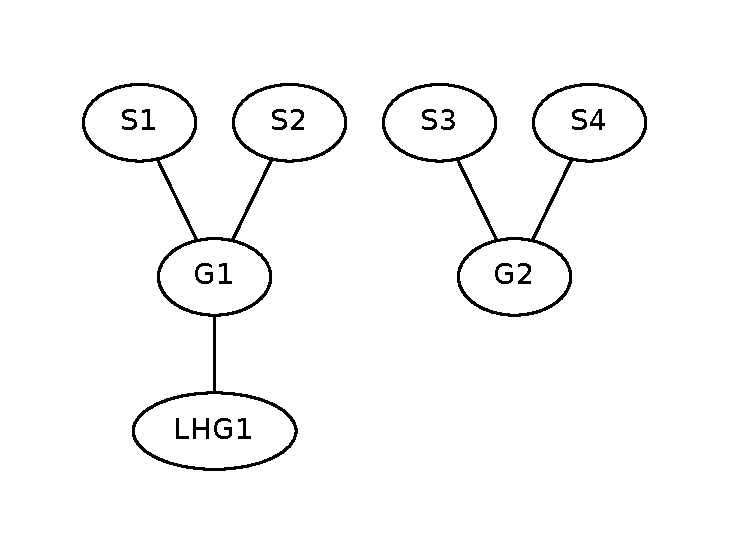
\includegraphics[width=7.0cm]{fig/labgroup/slack_add_2-5.pdf}        
  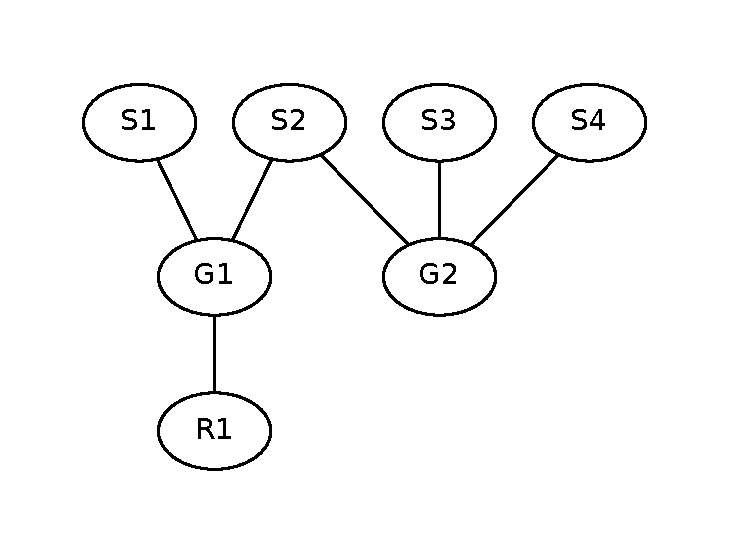
\includegraphics[width=7.0cm]{fig/labgroup/slack_add_3.pdf}        
  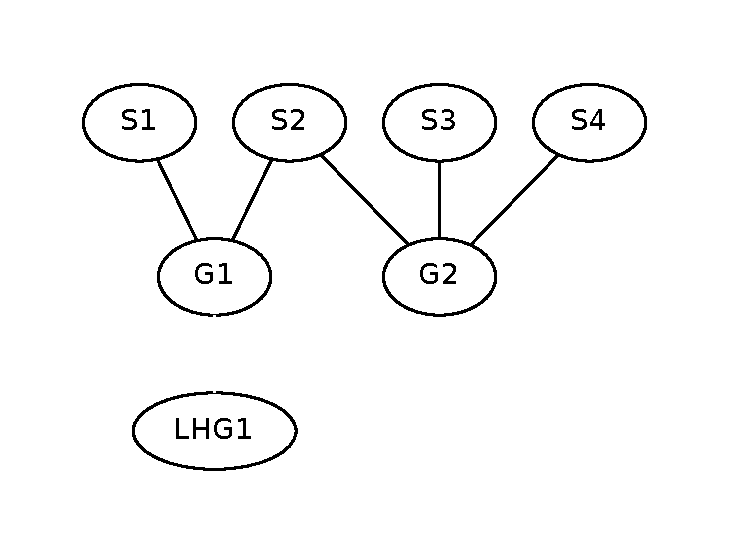
\includegraphics[width=7.0cm]{fig/labgroup/slack_add_4.pdf}        
  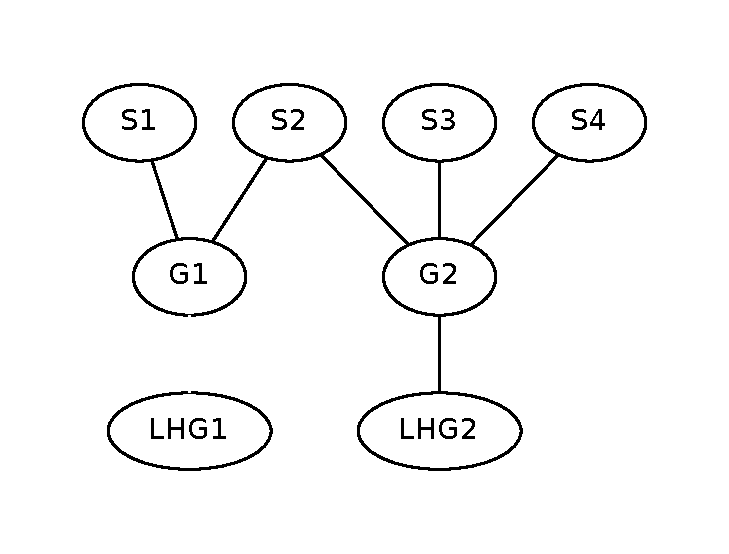
\includegraphics[width=7.0cm]{fig/labgroup/slack_add_5.pdf}        
  \caption[Serie tillstånd rörande labgrupper.]
  {Serie tillstånd rörande labgrupper. Studenterna $S2$, $S3$ och $S4$ vill
  bilda en nya laboraionsgrupp tillsammans (den som blev $G2$) där de ska skapa
  en LHG. Notera hur student $S2$ måste ta bort sin förra LHG innan någon elev
  kan lägga till en LHG i den nya gruppen. Mellan varje figur krävs att någon
  användare gör en åtgärd i waters system.}
  
\end{figure}

\subsection{Alltid exakt en LHG per laboration ($= 1$)}
\subsubsection{Förslag på implementering}
\paragraph{Initialtillstånd}
\paragraph{Operationer}
\subsubsection{Bevis av korrekthet}

 
\begin{figure}
  \centering
  \begin{subfigure}[b]{0.5\textwidth}
    \centering
    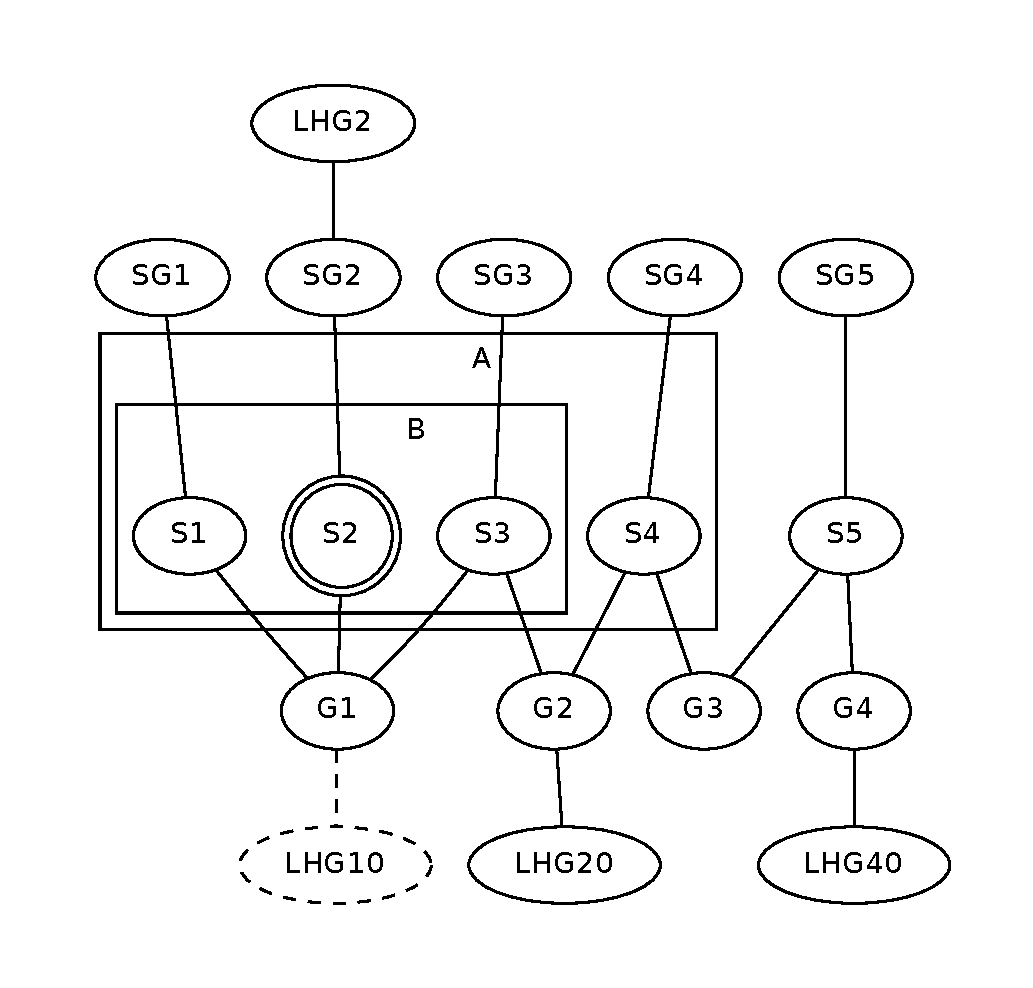
\includegraphics[width=8.0cm]{fig/labgroup/strict_proof.pdf}
    \caption{Situation när $S3$ ska lägga till $R20$}
    \label{fig:strict-proof}
  \end{subfigure}%
        ~ %add desired spacing between images, e. g. ~, \quad, \qquad etc. 
          %(or a blank line to force the subfigure onto a new line)
  \begin{subfigure}[b]{0.5\textwidth}
    \centering
    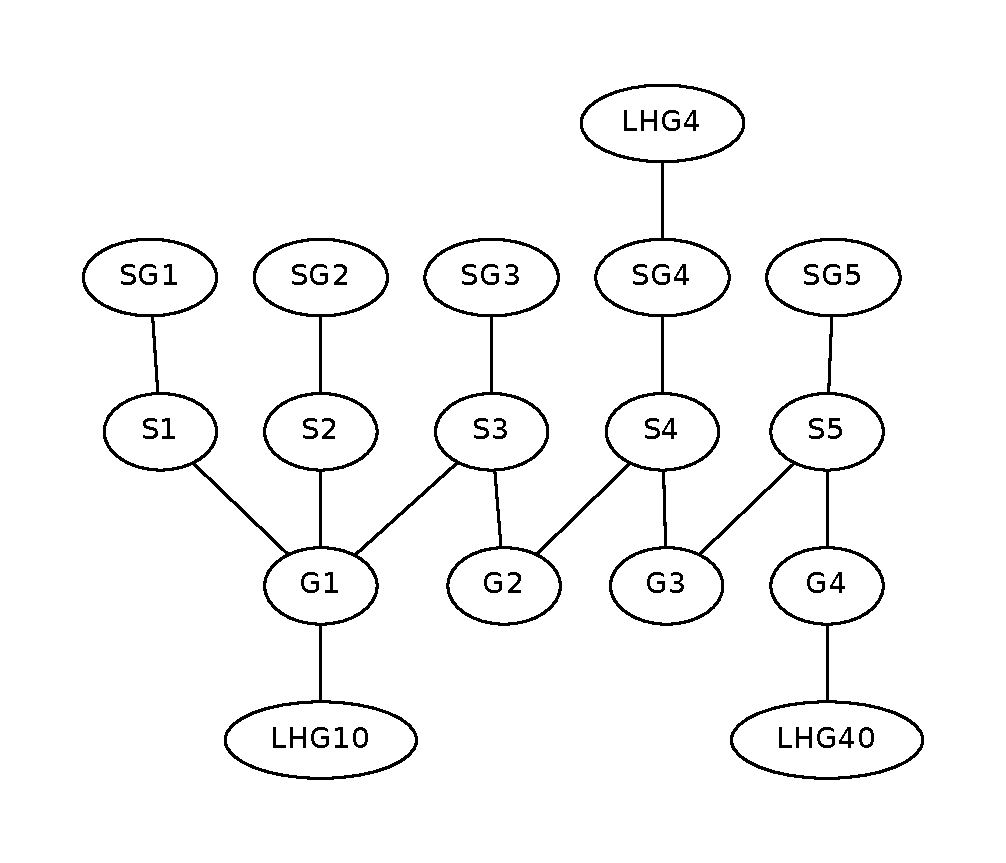
\includegraphics[width=8.0cm]{fig/labgroup/strict_proof_continue.pdf}
    \caption{Situation efter $R20$ lagts till}
    \label{fig:strict-proof-continue}
  \end{subfigure}
  \caption{Före och efter LHG-tillägg (strikt invariant)}\label{fig:animals}
\end{figure}

\subsubsection{Användarperspektiv}
\subsection{Ingen invaraint}
Hejsan hoppsan
